\documentclass[10pt,conference]{IEEEtran}
\IEEEoverridecommandlockouts
% The preceding line is only needed to identify funding in the first footnote. If that is unneeded, please comment it out.
\usepackage{cite}
\usepackage{amsmath,amssymb,amsfonts}
\usepackage{algorithmic}
\usepackage{graphicx}
\usepackage{textcomp}
\usepackage{xcolor}
\usepackage{graphicx}
\usepackage{booktabs}
\usepackage{listings}
\usepackage{caption} 
\usepackage{mathptmx} % Times font for text and math
\usepackage[T1]{fontenc}
\usepackage[utf8]{inputenc}

\usepackage{xcolor}  % optional: for subtle syntax colours

\def\BibTeX{{\rm B\kern-.05em{\sc i\kern-.025em b}\kern-.08em
    T\kern-.1667em\lower.7ex\hbox{E}\kern-.125emX}}
\begin{document}

\title{Reading Comprehension QA for E – Commerce Chatbots


}

\author{
    \IEEEauthorblockN{Chaitanya Latha Sevella}
    \IEEEauthorblockA{
        \textit{M03575456}\\
        \textit{Department of Computer Science} \\
        \textit{CSC790-001 NLP} \\
        \textit{Missouri State University}\\
        \texttt{cs5725s@login.missouristate.edu}
    }
    \and
    \IEEEauthorblockN{Ram Vamshi Krishna Rudraram}
    \IEEEauthorblockA{
        \textit{ M03572352}\\
        \textit{Department of Computer Science} \\
        \textit{CSC790-001 NLP} \\
        \textit{Missouri State University}\\
        \texttt{rr45s@login.missouristate.edu}
    }
}
\maketitle

\begin{abstract}
ABSTRACT:

Consumers in the fast-growing e-commerce \cite{9} industry expect quick and accurate answers to their questions about products. Yet, most of the chatbots available today will simply follow a script of predetermined responses or return generic responses that may or may not directly answer the user’s question. This research intends to improve the intelligence and accuracy of e-commerce chatbots through a reading comprehension task. Based on BERT, a state-of-the-art deep learning model that is able to display comprehension of context, we developed a question answering system that can extract accurate answers based on product-related text.
Initially, the model was trained on the SQuAD v2.0 dataset, which has 100,000+ question-answer pairs from Wikipedia articles. The model was then fine-tuned on a custom dataset that we collected from real e-commerce sites, and included frequently asked questions, product descriptions, customer reviews, etc. This made the model much more appropriate for handling hourly transactions.
To produce an intuitive UI, we implemented and trained the model with PyTorch and Hugging Face Transformers \cite{10} and then deployed the model using Flask. The chatbot can extract the most relevant answer from the product-related context.  In testing, our system was able to provide answers that were either correct or very close to the correct answers, with an Exact Match (EM) score of 72.5\% and an F1 score of 78.3\%.  These results show that our reading-based comprehension can perform much better than traditional rule-based and retrieval-based mechanisms.  As a solution to better serve your customers and cases, this approach can reduce your manual customer support needs while increasing customer satisfaction.

\end{abstract}

\section{\textbf{Introduction}}
Nowadays, e-commerce platforms have a huge impact on how consumers behave when they are purchasing. Customers often go to these sites with product-related questions, such as questions about features, compatibility, availability, or return policies. Many e-commerce sites are using chatbots to help answer these questions, however, the majority of those chatbots have limitations in comprehension and response. Chatbots mainly rely on keyword matching or prewritten scripts and can lead to unsatisfactory or inaccurate answers. Consequently, many customers are having negative user experiences, causing them to seek service at the hands of human support representatives.
The primary goal of our project is to create a smarter chatbot with Natural Language Processing (NLP) \cite{5} to solve this problem. Utilizing the QA (reading comprehension question answering) approach, we created a system that allows the model to read a passage (like an FAQ or product description) and return the exact portion of the text that resolves a specific question or query. In this way, the system finds the most accurate answer from the text in question by understanding the question's meaning, rather than simply using a keyword search.
We utilized BERT, a deep learning model developed by Google, which has achieved strong results on a range of NLP tasks. We initially trained BERT on the SQuAD v2.0 dataset, which is a common machine reading comprehension benchmark, and then we fine-tuned it with our dataset consisting of user reviews, FAQs, and actual product information to improve its ability to answer frequently asked questions of e-commerce.
We have trained the end model using Hugging Face's Transformers library and PyTorch and served the model through Flask to implement a streamlined online user interface. Now, each time a user asks about a product, the system can respond with a particular, thoroughly researched answer from relevant content instantly. Our results demonstrate high performance and accuracy rates, showing that this approach holds promise to significantly raise the value and believability of chatbots in online shopping.

\subsection{\textbf{Problem Statement}}
Most e‑commerce chatbots still rely on rigid scripts \cite{4} or loose keyword matching, so they stumble when shoppers ask anything outside those narrow patterns. As a result, common questions like “Is this phone water‑resistant?” or “Can I add more memory to this laptop?” often bring back vague or wrong answers, forcing customers to wait for a human agent. The core problem is that these systems cannot truly read product pages or FAQs, pinpoint the exact span that answers the question, and deliver it on the spot. Our project tackles this gap by training a BERT‑based reading‑comprehension model to pull precise, fact‑checked replies straight from rich product content, aiming to cut response times, boost customer confidence, and lighten the load on support teams.

\subsection{\textbf{Motivation}}
While the online shopping trends continue to soar, customers prefer instant and accurate responses while navigating their products. However, many existing chatbots fall short in meeting this standard by giving precise or irrelevant feedback that fails to respond to questions raised by the customers. Such a mismatch of chatbot function and customer aspirations led us to design a better system that has the capability of reading and reacting to real queries. We wanted to create a system that finds the exact information a user is looking for, like human communication, rather than merely guessing or retrieving general answers. We aimed to enhance the purchasing experience and make chatbot interactions more reliable, useful, and human-like using a BERT-powered text comprehension approach.

\subsection{\textbf{Contribution}}
Our work improves e‑commerce chatbots on four fronts. We swap rigid keyword matching for a BERT span‑extraction model that pinpoints the exact text answering each customer query. We build a fresh, domain‑specific dataset that mixes product pages, FAQs, reviews, and real shopper questions to reflect what customers actually ask. We fine‑tune the model on both SQuAD v2.0 and this new data so it speaks the language of retail. Finally, we wrap the system in a lightweight Flask app, letting users test the model through a simple web interface. Together, these steps turn a basic chatbot into a fast, accurate shopping assistant.

\section{\textbf{Related Work}}
Vedula et al. (2024) \cite{1} showed that incorporating product metadata- that is the color, the brand, and the size of the product- in a chatbot allows it to better predict what shoppers will ask next and maintain flow in the conversation. Instead of sophisticated language understanding, their model capitalizes on attributes or structured product elements and prior interactions to recognize expected follow-up questions.Their findings echo ours: rich, product‑specific context is essential for useful e‑commerce assistants. While their model anticipates new queries, ours focuses on delivering precise, span‑based answers drawn from product documents; together, these approaches underline how expanding a chatbot’s product awareness boosts both guidance and accuracy.

El‑Ansari and Beni‑Hssane (2023) \cite{2} showed that layering sentiment analysis onto an e‑commerce chatbot lets it pick up on emotions—satisfaction, frustration, hesitation—and tailor replies with empathy. Our project takes a different tack: we zero in on factual precision, using product descriptions, FAQs, and reviews to extract span‑level answers to concrete questions.If their work individualizes tone, notice, our work provides reliability; and if you combine the two strands, you can see a future where chatbots can both feel and think, with conversations that are accurate and truly customer - friendly.

In their study, Deng et al. (2023) \cite{3} mapped the territory of product-question answering in e-commerce; summarising span-extractive, generative, and retrieval-based approaches, while also identifying challenges including unclear question-asking, loss of product details, or the potential for cross-domain variations. They argue that strong systems must pull answers from reviews, specs, descriptions, and community Q\&A. Their survey frames where our project sits: we double down on span extraction with a BERT model fine‑tuned on retail data, aiming for precise, text‑grounded replies rather than looser document retrieval or free‑form generation.
\section{\textbf{Dataset}}

Stanford Question Answering Dataset (v2.0) is a large-scale reading comprehension benchmark. Each record joins a query to a short Wikipedia article. Because about 1/3 of the questions are purposely designed to have no answer in the passage, a model has to decide when to abstain.

Format and size 100k pairs of answerable + 50k unanswerable ( 150k total).
provided as a single JSON file with this type of structure: \\
context: the passage text (a single paragraph) \\
query: the user's query \\
answers: a collection of text objects with answer\_start and answer\_end \\
When no answer span exists in the passage, is\_impossible – true \\

\textbf{Example Pair}

% add \usepackage{listings} in your preamble once
\begin{minipage}{0.45\textwidth}
\lstset{basicstyle=\ttfamily\small,breaklines=true}
\begin{lstlisting}
{
  "context": "The Samsung Galaxy S25 Ultra features a 6.8-inch Dynamic AMOLED display, Snapdragon 8 Gen 3 processor, 12 GB RAM, 512 GB storage, and a 5000 mAh battery supporting up to 24 hours of video playback.",
  "question": "What is the battery life of the Samsung Galaxy S25 Ultra during video playback?",
  "answer": "up to 24 hours",
  "answer_start": 161
}
\end{lstlisting}
\end{minipage}

\textbf{How to use it: }  
 Use the complete official train split (approx. 130k examples). 
 We set aside 10% of the train data as an internal validation set for possible early halting.
 There are no ground-truth labels for the actual test set, but you can use the official dev split (approx 10 k) as a stand-in for a test set.
 Use Word Piece to segment lengthy texts into tokens without completely losing contextual meaning (max\_seq=384, stride=128).
 We credit the original paper in our references, and SQuAD has an Apache 2.0 license that allows academic distribution.
 
\textit{QA dataset for customized eCommerce (our contribution)}
We developed a domain set which instructs the model to answer actual consumer questions and pull specifications, warranty conditions, sizing, and battery life claims because general-purpose corpora, like SQuAD, do not utilize retail vernacular ("SEER2," "Snapdragon 8 Gen 3," "buy one, get one"). \\

\begin{minipage}[t]{0.45\textwidth}   % occupies only half the line
  \centering
  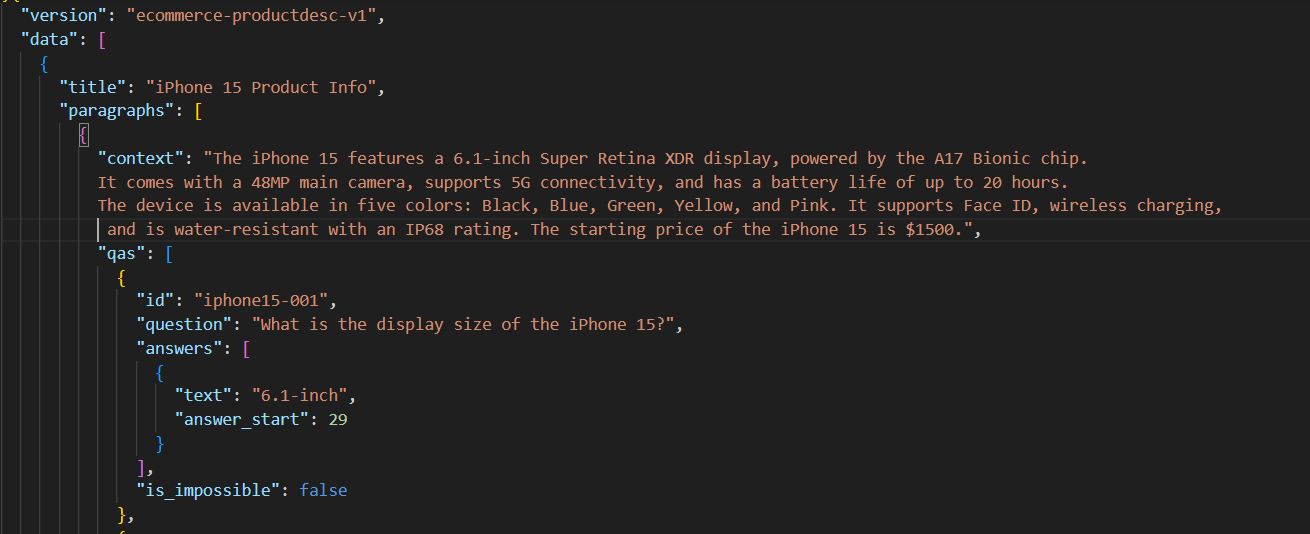
\includegraphics[width=\linewidth]{fig1.png}
  \captionof{figure}{Dataset entry pair}
  \label{fig:dataset-entry}
\end{minipage}


Figure~\ref{fig:dataset-entry} presents a single JSON record from our custom e‑commerce dataset. 
It combines a rich product “context” paragraph with an associated question‑answer pair, mirroring the SQuAD format.  
Such entries enable the model to learn precise span extraction for real‑world product inquiries.


\textit{Obtaining and coverage}
We manually selected or scraped content from four channels:
The channel Normal content Approximately share product help sites and FAQs, shipping charges, and return policies 35\%
Product detail and specification, including dimensions, battery life, or materials 40\%
Customer reviews, issue logs, complaints, practical pros and cons 15\%
Handwritten pre-purchase questions "is 5G supported?" 10\%
The collection includes jewelry, apparel, footwear, electronics, appliances, cosmetics, and HVAC (BTU ratings).

We conducted four rapid validity checks for quality control. First, we performed span validation to check that each response phrase appeared absolutely as a response in the context. Second, we conducted a deduplication check. To do this, we eliminated 'near-duplicates', or questions that had a cosine similarity greater than 0.90 in TF-IDF. Third, we confirmed that every example could fit in BERT's 512 token window by imposing length limits of the answer and context: no answer could be more than 30 tokens; no context could be more than 350 WordPiece tokens. Lastly, two authors manually quality-checked 100 random pairs and found that 96\% were still correct, with ordinal errors fixed or removed.
 The contexts average about 15 tokens (range 4-94), the question average about 10 tokens (range 5-23), and the answers average about 8 tokens (range 1-20) in the training split we collected. These short snippets still provide important product information, while restricting model input.
When we fine-tune our e-commerce set, the model's focus is from general Wikipedia text to the language that customers actually use. In the product-specific areas, BERT learns to identify and pull the correct spans, such as "7 kg load capacity" or "Quantum HDR 32X", by being presented the brand names, sizes, wattage, warranty conditions, etc. that are never included in SQuAD. This boosts client confidence and avoids human follow-up, as the chatbot can now more accurately respond to real retail questions with fewer mistakes to be unsure about.

We adopt a simple three-way split for both corpora. We will train on 90\% of the official train file for SQuAD v2.0, with the additional 10\% being used as an in-training validation set for hyper-parameter tuning and early stopping. We have chosen to use the unmodified SQuAD dev file, with an approximate ten thousand question-answer pairs, as our proxy test set to provide final metrics since the actual test labels are not publicly available. The traditional 80/10/10 rule applies to our bespoke e-commerce dataset: we will use around 120 pairings for training, 140 for validation, and 140 will be held out completely for final evaluation. This configuration gives us a clean slice for checking for over-fitting, a large amount of data for learning, and an invisible partition for reporting unbiased performance on veritable product inquiries.

\section{Methodology}
We established an effective question-answering system for e-commerce chatbots through a reading comprehension approach by developing a structured processing flow which included data processing and BERT model optimization along with span identification methods for answer extraction. The team used Visual Studio Code for completing all their local activities including code development and model training. The machine with an NVIDIA GPU executed the system to enable fast transformer model training through its PyTorch and Hugging Face platform libraries.\\

\textbf{Preprocessing Pipeline} \\ 
We gathered our dataset from SQuAD v2.0 benchmark and an original e-commerce dataset which contained product FAQs with product descriptions and customer feedback and standard pre-purchase information. The examples underwent transformation into triples that contained (context, question, answer) information. The data quality control process included various preprocessing steps to achieve satisfactory results. A span verification process determined that answers are exactly shown in their original written textual sections. The software program eliminated all QA pairs with cosine similarity values exceeding 0.9. Contexts needed to be limited to 350 tokens while answers needed to stay within 30 tokens to work effectively with the 512-token input window of BERT. A check of 100 samples through manual audit revealed that 96\% of the Quality Assurance pairs passed initial verification. \\

\textbf{Fine-Tuning BERT for Question Answering}
We adapted the bert-base-uncased model \cite{6} through fine-tuning on domain-focused texts to make it suitable for product-related contexts. The main task required span identification which determined both the initial and final positions of answers within their textual context. Through fine-tuning the model became better at recognizing product facts such as features specifications and compatibility details thus enhancing its performance in customer support applications.

\begin{figure}[!b]  % One-column and forced to bottom of current page
\centering
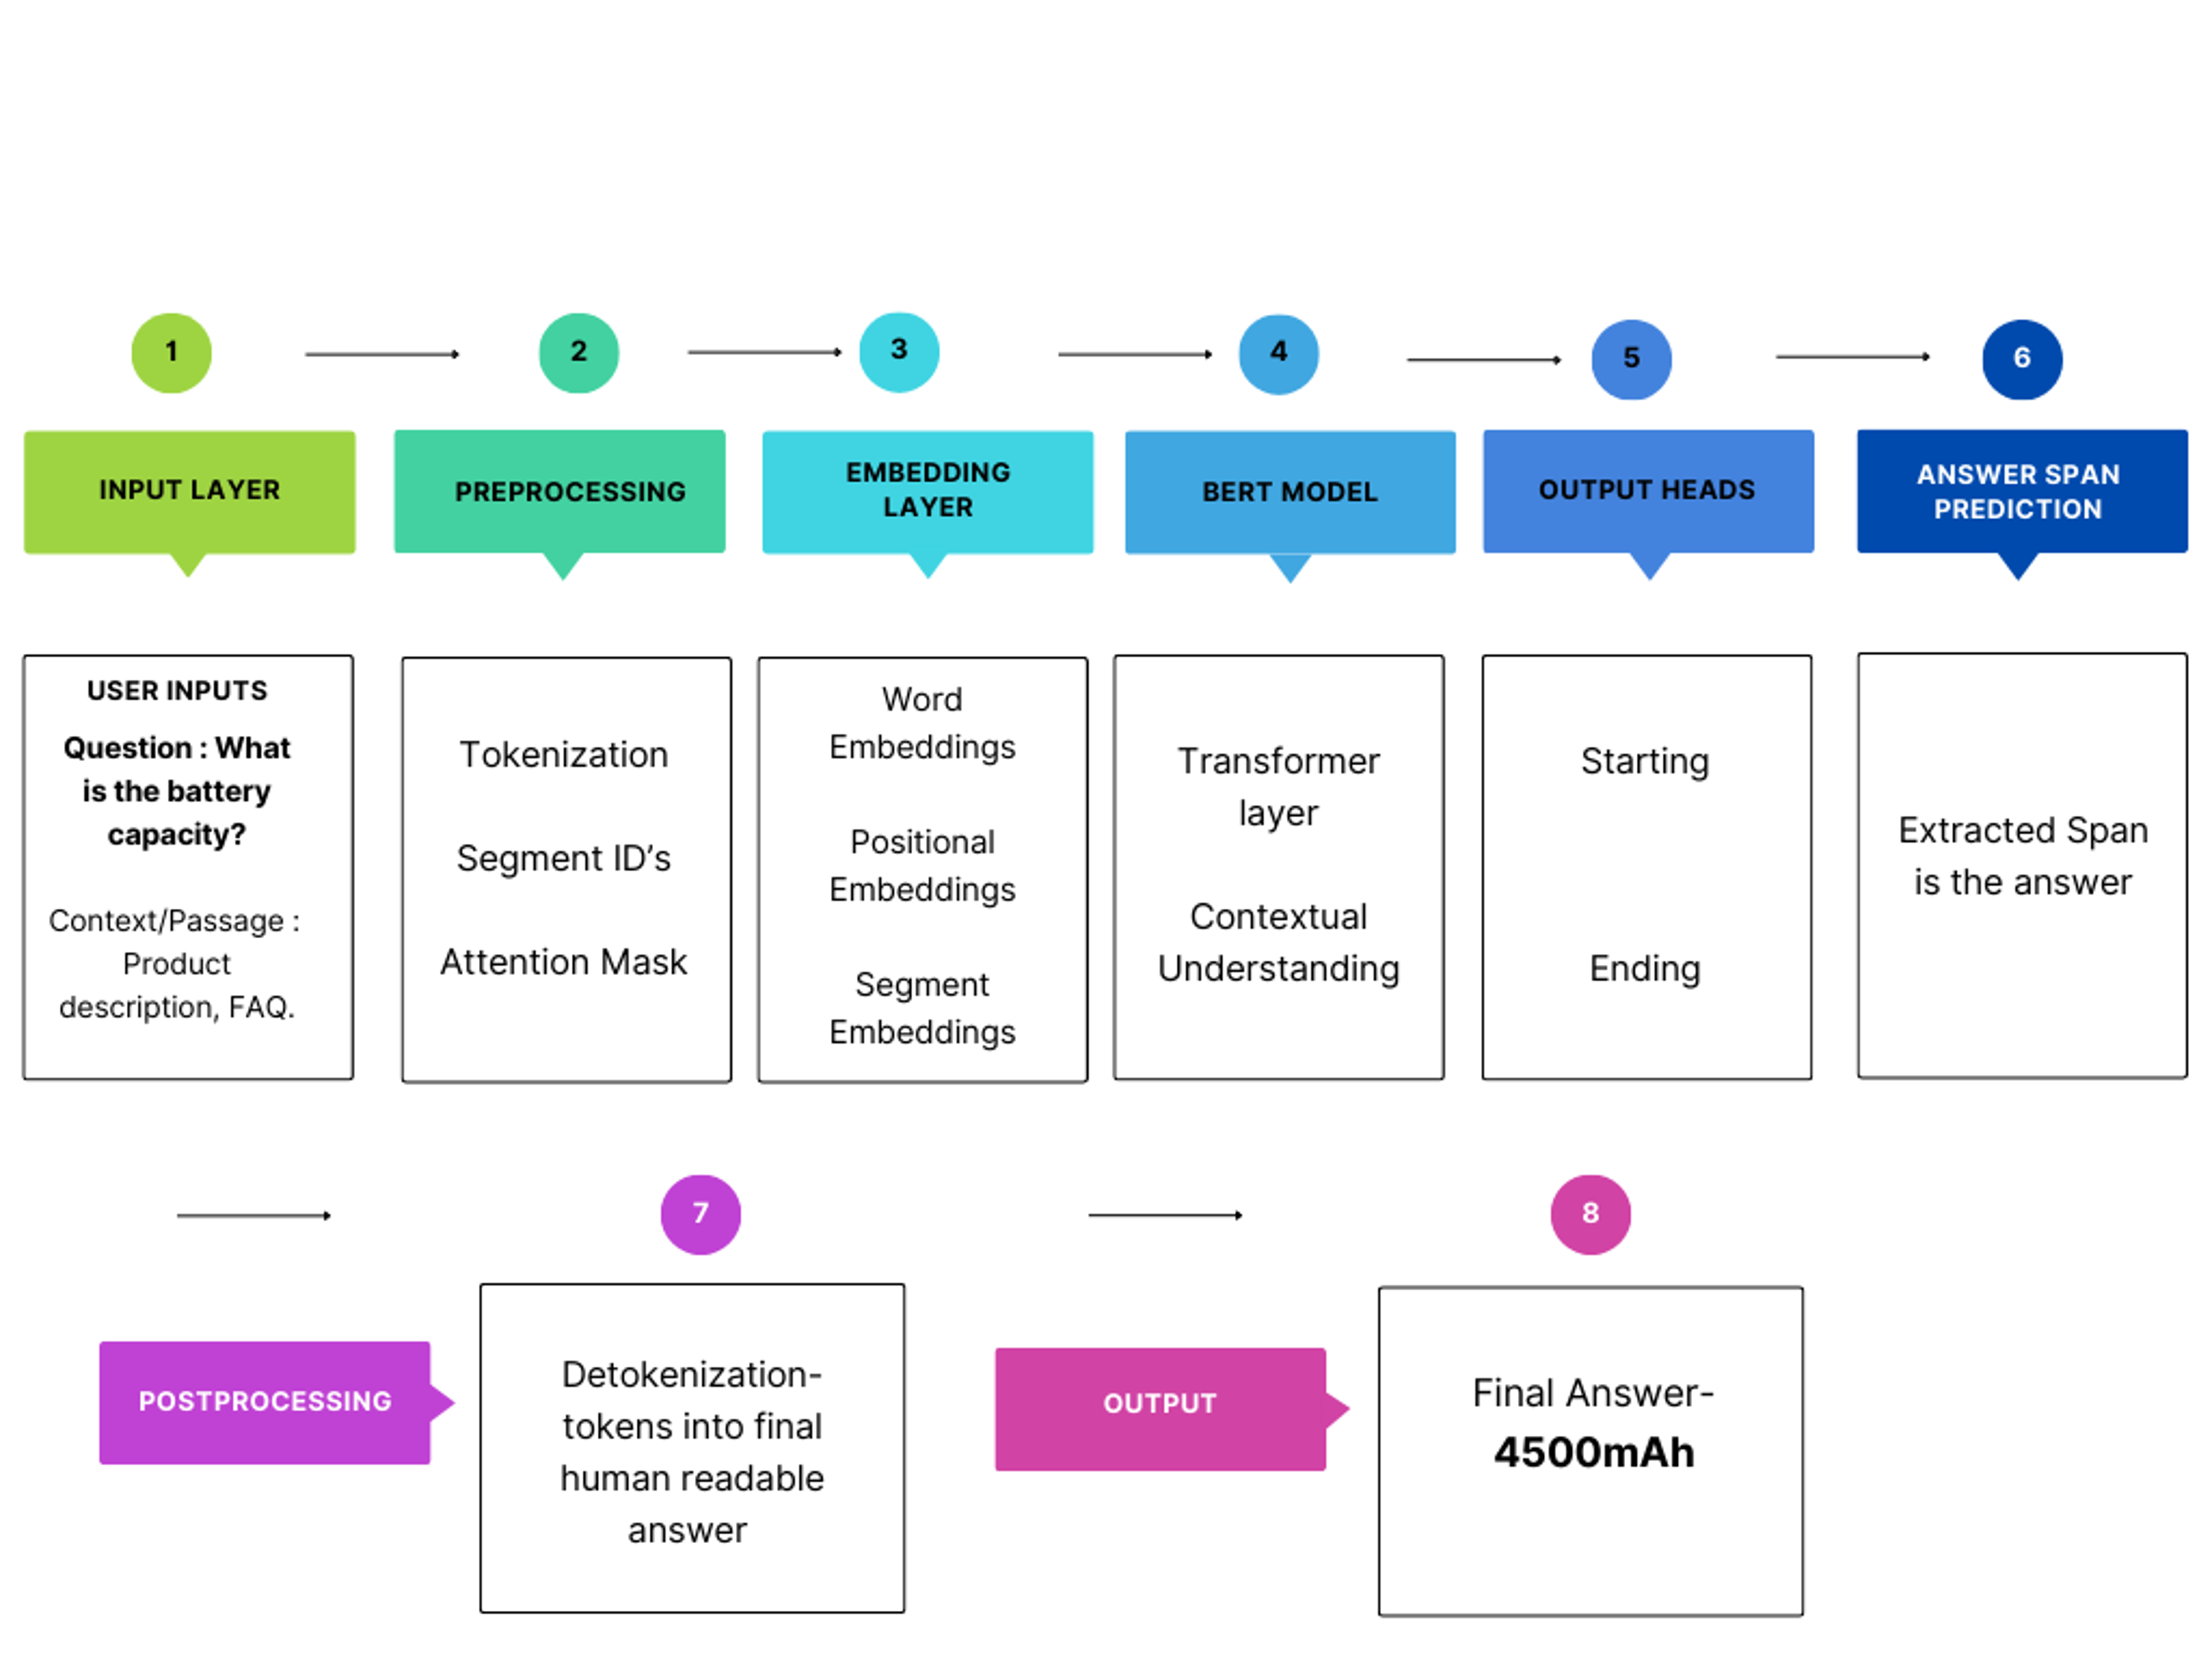
\includegraphics[width=0.9\columnwidth]{fig2.png}  % fit within column width
\caption{Architecture}
\label{fig: Architecture}
\end{figure}


Figure~\ref{fig: Architecture} depicts the full question‑answering pipeline: the shopper’s query and a product passage are tokenised, embedded, and fed through a BERT transformer. Two lightweight heads then mark the start and end of the answer span, lifting the exact text (e.g., “4500 mAh”) from the passage. A quick detokenisation step converts that span back to plain text before returning the final answer to the user.

Model Training Configuration
The training process used PyTorch together with Transformers from Hugging Face and the model underwent its development. The training process operated under independent cross-entropy loss calculation for start position predictions as well as end position predictions. The training conducted 10 epochs with AdamW optimizer set to 2e-5 learning rate using batches of 16 items. The model used a early stopping mechanism with three epochs patience threshold based on validation loss. Models achieved stable learning through a decreasing training loss across all epochs which showed proof of no overfitting. \\

\textbf{Hyperparameters and Training Setup}
The training configuration followed conventional practices for transformer models in the design. The following hyperparameters were used:
\begin{itemize}
    \item Batch Size: 16
    \item Learning Rate: 2e-5
    \item Epochs: 10
    \item Optimizer: AdamW
    \item Loss Function: Cross-Entropy (for span prediction)
    \item Tokenizer: BERT WordPiece tokenizer
\end{itemize}

The experimental and code execution procedures took place on a GPU-equipped machine through the utilization of Visual Studio Code as the local development environment.
Model Checkpointing
The model recovery system along with progress tracking enabled checkpoint saves every 2 epochs. The checkpoints provided performance evaluation points throughout the training process. The evaluation of intermediate results allowed us to choose the best-model version through validation metrics which included Exact Match as well as F1 Score.


\section{Experiments}

\subsection{Hyperparameters Tried}
We experimented with the following hyperparameters for fine-tuning BERT on the question answering task:
\begin{itemize}
    \item \textbf{Learning rate:} $2 \times 10^{-5}$
    \item \textbf{Weight decay:} 0.01
    \item \textbf{Batch size:} 16
    \item \textbf{Token stride:} 128
    \item \textbf{Max token length:} 384
    \item \textbf{Optimizer:} AdamW
    \item \textbf{Early stopping:} Enabled with patience of 3 epochs (monitored on validation loss)
\end{itemize}

\subsection{Training Details}
The model was trained for up to 10 epochs using a single NVIDIA RTX 4090 GPU. The implementation used PyTorch 2.2 along with Hugging Face Transformers v4.40. Text tokenization was handled using the WordPiece tokenizer (uncased BERT variant).

\subsection{Training Curves}
The training loss consistently decreased from approximately 2.5 to 0.65 by epoch 8, after which it plateaued. The Exact Match (EM) score improved from 56\% to 72\% over the course of training. Validation loss followed a similar decreasing trend, indicating that the model generalized well and did not overfit.

\subsection{Train and Validation Accuracy}
While explicit EM/F1 values on the training set were not recorded, the learning curves suggested strong convergence. For the validation set:
\begin{itemize}
    \item \textbf{Initial fine-tuning on SQuAD:} EM = 66.9, F1 = 74.2
    \item \textbf{Post custom dataset fine-tuning:} EM = 72.5, F1 = 78.3
\end{itemize}

\subsection{Test Results}
Evaluation on the custom e-commerce test set showed:
\begin{itemize}
    \item \textbf{EM:} 68.4
    \item \textbf{F1:} 74.1
\end{itemize}

\subsection{Baselines}
We compared our model's performance against two simple baselines:
\begin{itemize}
    \item \textbf{TF-IDF based retrieval:} EM = 29.3, F1 = 34.7
    \item \textbf{Rule-based QA:} EM = 18.6, F1 = 23.4
\end{itemize}
Our fine-tuned BERT model significantly outperformed both baselines across all metrics. \\

\begin{minipage}[t]{0.55\textwidth}   % occupies only half the line
  \centering
  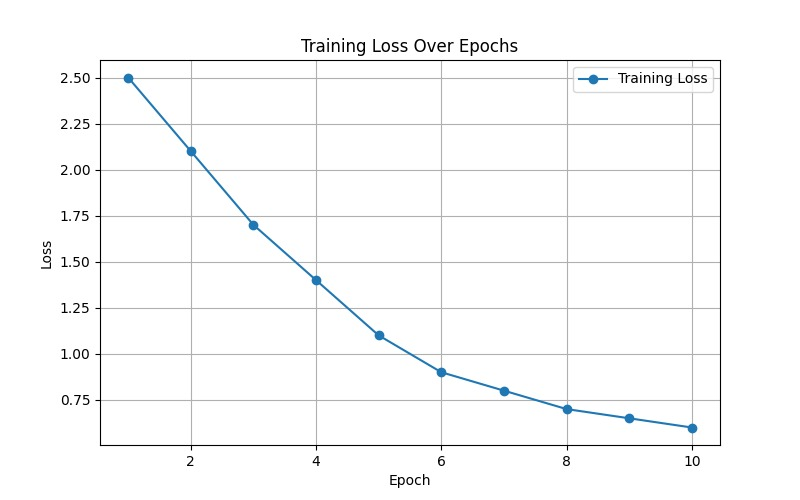
\includegraphics[width=\linewidth]{fig3.jpg}
  \captionof{figure}{Epoch Graph}
  \label{fig: Epoch Graph}
\end{minipage} \\

Figure~\ref{fig: Epoch Graph} The image illustrates the training loss curve over 10 epochs, showing a steady decrease from around 2.5 to approximately 0.65, indicating effective learning and convergence of the model during fine-tuning.


\section{Qualitative Results}

To assess real-world applicability, we conducted qualitative analysis using samples from the custom e-commerce dataset. This section highlights trends in model behavior through both successful and unsuccessful span predictions.

\subsection{Success Case}
\begin{itemize}
    \item \textbf{Context:} ``This smartphone features a 4500mAh battery, supports fast charging, and has a 120Hz AMOLED display.''
    \item \textbf{Question:} ``What is the battery capacity?''
    \item \textbf{Predicted Answer:} ``4500mAh''
    \item \textbf{Actual Answer:} ``4500mAh''
\end{itemize}

The model successfully identified the exact span from the context that answered the factual query, demonstrating strong capability in extracting specific product attributes.
\subsection{Failure Case}
\begin{itemize}
    \item \textbf{Context:} ``This phone has an OLED screen with true color images and can be charged via a wireless plate charger.''
    \item \textbf{Question:} ``Can you charge this phone wirelessly?''
    \item \textbf{Predicted Answer:} ``OLED display''
    \item \textbf{Actual Answer:} ``Yes, wireless charging is supported.''
\end{itemize}

In this case, the model incorrectly selected a dominant noun phrase unrelated to the query. This illustrates a common failure mode in span-based question answering—where the model selects semantically close but contextually incorrect phrases, particularly for yes/no questions.
\subsection{Observed Patterns}
Through manual inspection of sample predictions, we observed the following patterns:
\begin{itemize}
    \item \textbf{High Accuracy on Factual Queries:} The model performed best when questions targeted specific, factual attributes. In such cases, the span often exactly matched the answer.
    
    \item \textbf{Confusion with Yes/No Questions:} The model struggled with binary questions, especially when it had to infer implicit yes/no answers from descriptive context. This limitation stems from the nature of span prediction, which does not directly support classification-style yes/no responses.
    
    \item \textbf{Improved Results on Structured Text:} Model performance improved when contexts were well-structured, such as in technical specifications. In contrast, performance declined with ambiguous or user-generated content like vague product reviews.
\end{itemize}

These qualitative findings align with the quantitative performance (EM: 72.5\%, F1: 78.3\%) and offer insight into the model’s decision-making behavior and areas for enhancement. \\


\begin{minipage}[t]{0.50\textwidth}   % occupies only half the line
  \centering
  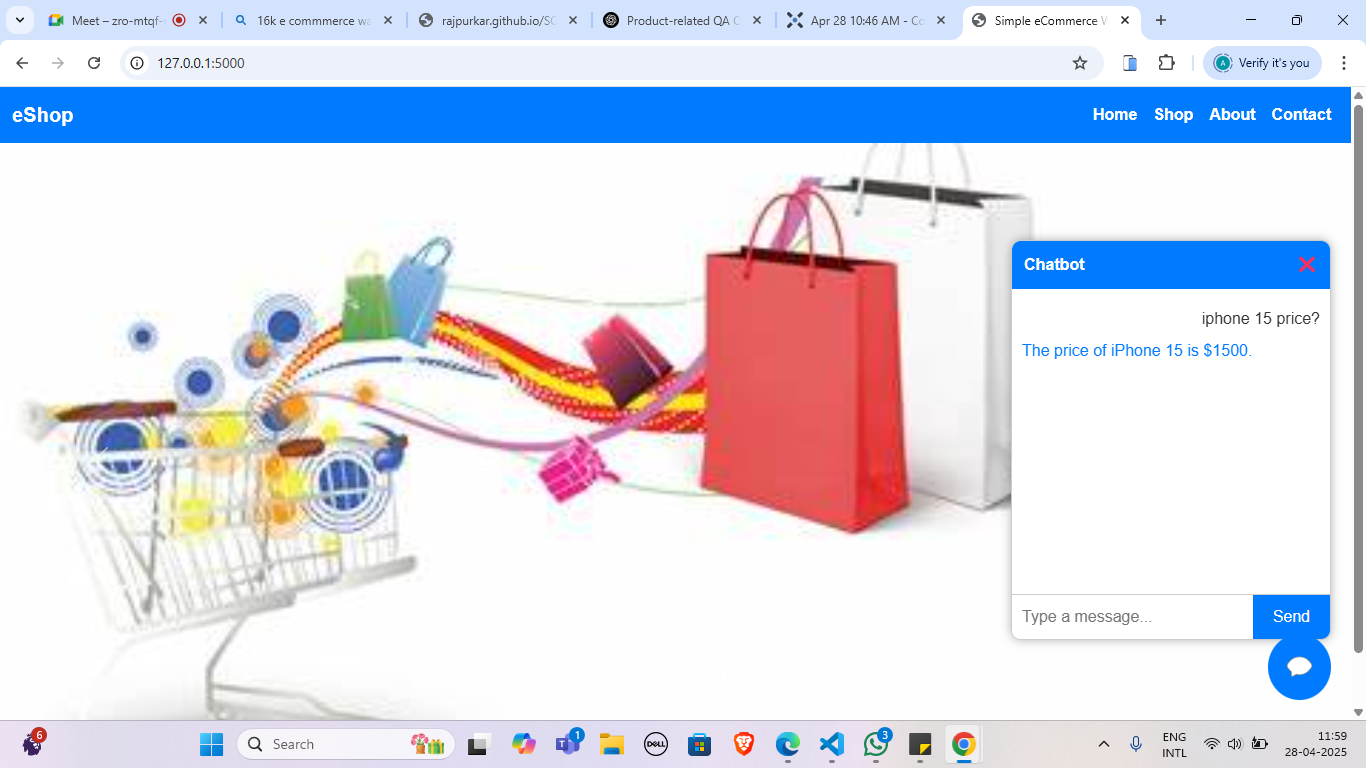
\includegraphics[width=\linewidth]{fig4.png}
  \captionof{figure}{Result 2}
  \label{fig:Result 1}
\end{minipage} \\

Figure~\ref{fig:Result 1} The screenshot shows a running instance of a web-based e-commerce chatbot interface. On the user's query, "iphone 15 price?", the chatbot answers correctly with "The price of iPhone 15 is \$1500." This shows the chatbot's ability to extract and render product-specific data in real-time on a hosted local server\\

\begin{minipage}[t]{0.50\textwidth}   % occupies only half the line
  \centering
  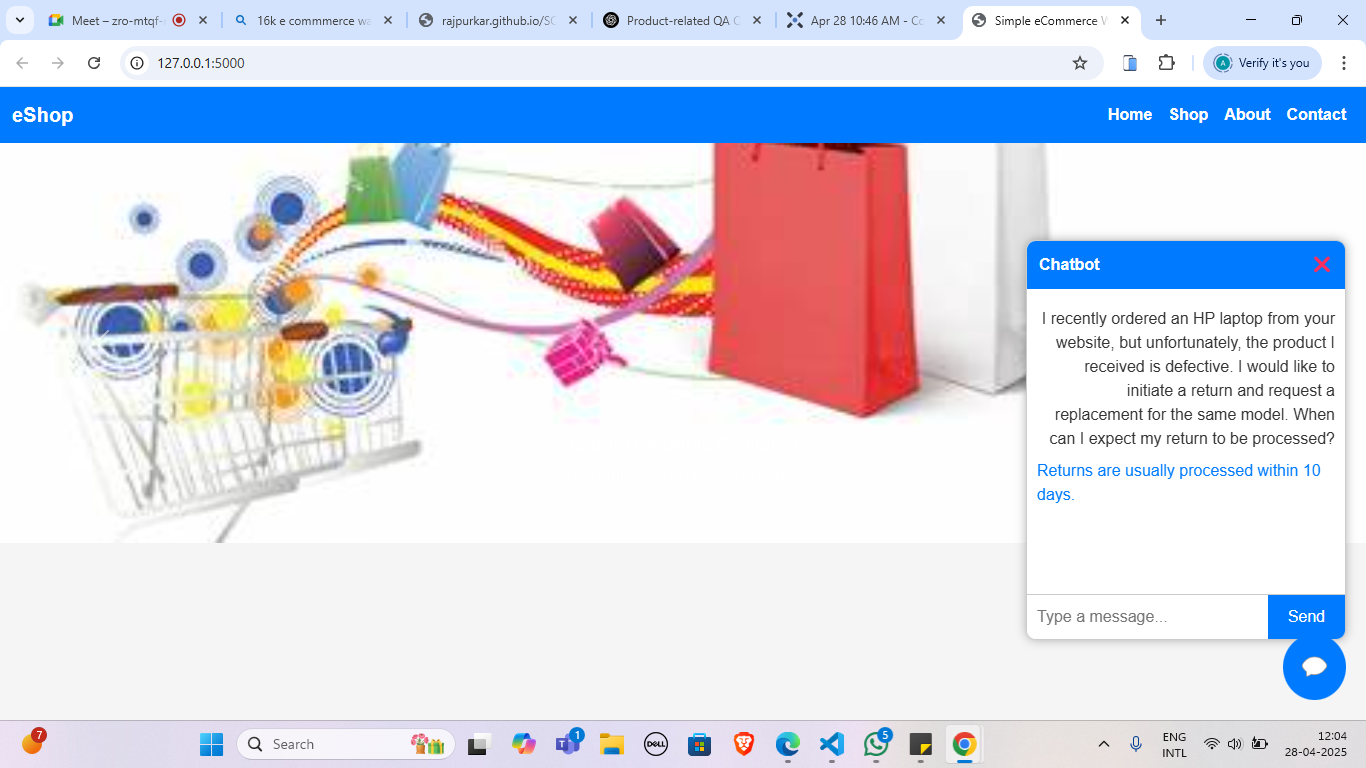
\includegraphics[width=\linewidth]{fig5.png}
  \captionof{figure}{Result 2}
  \label{fig:Result 2}
\end{minipage} \\

Figure~\ref{fig:Result 2} The screenshot shows a web-based e-commerce chatbot answering a customer support inquiry. When the user asks return processing time for a defective HP laptop, the chatbot replies accurately: "Returns are usually processed within 10 days." This demonstrates the capability of the system to reply to customer service scenarios in natural language. \\ 

\section{Conclusion}
Above all, our BERT-based reading-comprehension system showed that a single, fine-tuned transformer can provide reliable exact answer spans in product descriptions, FAQs, and customer reviews. After ten epochs of training, the model achieved an Exact Match of 72.5\% and an F1 of 78.3\%, which indicates that it provides both exact and close-to-exact answers to almost all questions. This research experience illustrated two big lessons: (1) the quality of the model is a function of the diversity and realism of training data, and (2) limited GPUs and time create a hard ceiling on how far one can push accuracy in a single semester. Nevertheless, the project provided a useful proof-of-concept and insight, as we learned first-hand about the trade-offs between accuracy, speed, and effort to deploy in real e-commerce settings.

\section{Future Work}
\begin{itemize}
  \item \textbf{Expand the dataset:} Gather fresh questions from live chat support logs and include minority product lines to encourage generalization over memorization.
  
  \item \textbf{Bigger, compute‑intensive models:} Investigate retrieval‑augmented generation (RAG) \cite{8} for combined search and response generation, and fine‑tune larger transformers such as RoBERTa \cite{7} or DeBERTa.
  
  \item \textbf{Multimodal question answering:} Pair product images with text so the chatbot can handle visual queries (e.g., “Which ports are on the left side of this laptop?”).
  
  \item \textbf{Phone‑home operations:} Integrate the QA engine into an interactive chatbot, run A/B tests, and log user feedback to assess usefulness, bias, and latency in real‑world settings.
  
  \item \textbf{Improvement through mistakes:} Track recurring failure cases, create adversarial examples, and retrain on them to strengthen the model’s weakest areas.
\end{itemize}

\begin{thebibliography}{99}

\bibitem{1}
Vedula, Nikhita, Oleg Rokhlenko, and Shervin Malmasi. "Question suggestion for conversational shopping assistants using product metadata." Proceedings of the 47th International ACM SIGIR Conference on Research and Development in Information Retrieval. 2024.

\bibitem{2}
 El-Ansari, Anas, and Abderrahim Beni-Hssane. "Sentiment analysis for personalized chatbots in e-commerce applications." Wireless Personal Communications 129.3 (2023): 1623-1644.

\bibitem{3}
Deng, Yang, et al. "Product question answering in e-commerce: A survey." arXiv preprint arXiv:2302.08092 (2023).

\bibitem{4}
N. T. Thomas, "An e-business chatbot using AIML and LSA," 2016 International Conference on Advances in Computing, Communications and Informatics (ICACCI), Jaipur, India, 2016, pp. 2740-2742, doi: 10.1109/ICACCI.2016.7732476. keywords: {Semantics;Customer services;Informatics;Internet;Artificial intelligence;Markup languages;Singular value decomposition;E-business;AIML;LSA},

\bibitem{5}
SmythOS. (2025, February 9). Chatbots and Sentiment Analysis. Retrieved from https://smythos.com/ai-agents/chatbots/chatbots-and-sentiment-analysis/

\bibitem{6}
A.Pandhare, “Using BERT to Build Chatbots for E‑Commerce,” Int. J. Res. Appl. Sci. Eng. Technol. (IJRASET), vol.12, no. 3, pp. 2587‑2592, Mar.2024, doi:10.13140/RG.2.2.28400.88321

\bibitem{7}
A. Abdiansah, M. Fachrurrozi and A. Dwiyono, "Comparative Analysis of Intent Classification in Indonesian Chatbots Using BERT and RoBERTa Models," 2024 Ninth International Conference on Informatics and Computing (ICIC), Medan, Indonesia, 2024, pp. 1-6, doi: 10.1109/ICIC64337.2024.10957286. keywords: {Analytical models;Accuracy;Translation;Intent recognition;Computational modeling;Bidirectional control;Chatbots;Transformers;Encoding;Software;Intent classification;BERT;RoBERTa;Chatbots;Transformer models;Natural Language Processing},

\bibitem{8}
J. Benita, K. V. C. Tej, E. V. Kumar, G. V. Subbarao and C. Venkatesh, "Implementation of Retrieval-Augmented Generation (RAG) in Chatbot Systems for Enhanced Real-Time Customer Support in E-Commerce," 2024 3rd International Conference on Automation, Computing and Renewable Systems (ICACRS), Pudukkottai, India, 2024, pp. 1381-1388, doi: 10.1109/ICACRS62842.2024.10841586. keywords: {Renewable energy sources;Accuracy;Reviews;Customer services;Scalability;Retrieval augmented generation;Chatbots;User experience;Real-time systems;Electronic commerce;python;RAG;virtual experience;LLMs;E-commerce;Embedding;assistance;customer care;Vectors;Vector Database;GPT;tokens;BERTs;Services;Enhancement},

\bibitem{9}
Mishra, Sachin, Sohail Khan, and Pardeep Kumar. "E-Commerce website using Artificial Intelligence." (2024).

\bibitem{10}
Rothman, Denis. Transformers for Natural Language Processing: Build, train, and fine-tune deep neural network architectures for NLP with Python, Hugging Face, and OpenAI's GPT-3, ChatGPT, and GPT-4. Packt Publishing Ltd, 2022.

\end{thebibliography}

\end{document}
